\chapter{Attraversamento}

\paragraph{Problema:} Il problema dell'attraversamento consiste nell'avere una
configurazione iniziale dove tutte le entità sono nello stesso stato (IDLE)
eccetto una che sarà l'unico iniziatore. L'obiettivo è quello di visitare una
alla volta tutte le entità in maniera sequenziale. Il messaggio che dovrà
transitare tra le entità si chiama TOKEN (T).

\paragraph{Formalmente:}

$$
    P_{INIT} = <\exists ! x \in \xi | Value(x) = T \;>
$$

OVVERO: Esiste una sola entità all'interno del sistema che possiede il
Token T, tutte le altre saranno in stato di Idle.

$$
    P_{FINAL} = <\exists t>0 | \forall x \in \xi \exists t' \leq t | value_{t'}(x)
    = T \text{ and } value_{t'}(y) \neq T, \forall y \neq x >
$$

\textit{Ovvero:} Esiste un tempo t maggiore di 0 tale per cui per ogni $t' \leq
    t$ c'è una sola entità che detiene il token e per ogni entità esiste un tempo
$t'' \leq t$ nel quale X è proprio la detentrice del token e nessun altra lo
possiede.

\paragraph{Restrizioni:} R, UI (iniziatore unico che detiene il Token).

\paragraph{Tipologie di messaggi inviati:}
\begin{itemize}
    \item T : Messaggio di Token
    \item Return: Inviato da un nodo per avvertire il padre che il sottografo è
          stato completamente esplorato.
    \item Back\_Edge : T viene inviato ad un nodo che è già stato visitato,
          quell'arco viene catalogato come Back\_edge e da li non passeranno mai più
          token.
\end{itemize}

\paragraph{Stati possibili dell'algoritmo:}
\begin{itemize}
    \item Idle
    \item Initiator
    \item Visited
    \item Done
\end{itemize}

\paragraph{Caratteristica dell'algoritmo e differenza con il Broadcast:} Si
effettua una visita sequenziale delle entità. Ovvero un'entità alla volta può
possedere il Token T, quando un nodo riceve T, esso è marcato come "Visited".

\section{Funzionamento dell' algoritmo tramite DFS}
\begin{enumerate}
    \item Quando un'entità riceve per la prima volta il TOKEN, cambia stato in
          VISITED e crea l'insieme "Unvisited" che contiene tutti i suoi vicini tranne
          l'entità che gli ha spedito il token. Manda poi il TOKEN verso un nodo
          nell'insieme, lo rimuove da quest'ultimo e aspetta il messaggio di RETURN.
    \item Quando uno dei vicini riceve il TOKEN:
          \begin{itemize}
              \item Se è già stato visitato (VISITED), manda indietro un messaggio
                    di BACK\_EDGE per poi rimuove il sender dal suo vicinato (così che non
                    potrà inviargli T nemmeno per sbaglio).
              \item Altrimenti cambia stato in VISITED e spedisce il TOKEN
                    sequenzialmente ad ogni suo vicino non visitato e successivamente
                    manda il messaggio di RETURN verso il padre.
          \end{itemize}
    \item Dopo la ricezione del RETURN, un'entità manda il TOKEN ad un altro
          vicino localmente non visitato.
    \item Se non ci sono più vicini disponibili, allora manda RETURN a sua volta.
\end{enumerate}

Quindi, l'insieme degli Unvisited viene aggiornato quando:
\begin{itemize}
    \item Un'entità manda il token
    \item Viene inviato un Backedge (ho sbagliato strada ma aggiorno comunque il
          mio insieme degli Unvisited per non sbagliare nuovamente).
\end{itemize}

\subsection{Protocollo DFTraversal}
\begin{lstlisting} [caption={\textit{Protocollo DFTraversal.}}]
S = {INITIATOR, VISITED, IDLE, DONE}
$S_{INIT}$ = {INITIATOR, IDLE}
$S_{START}$ = {INITIATOR}
$S_{TERM}$ = $S_{FINAL}$ = {DONE}

Restrictions = RI+

INITIATOR
    Spontaneously
    begin
        Unvisited := N(x)
        initiator := true // serve per terminare il protocollo
        VISIT
    end

Procedure VISIT 
    begin
        if unvisited != 0 then
            next <- unvisited
            send(T) to next
            become VISITED
        else
            become DONE
            if not initiator then 
                // a chi mi ha raggiunto la prima volta
                send(RETURN) to entry
    end

IDLE 
    Receiving(T)
    begin
        unvisited := N(x) - sender
        entry := sender
        initiator := false
        VISIT
    end

VISITED
    Receiving(T)
    begin
        send(BACK_EDGE) to sender
        Unvisited := Unvisited - sender
    end

    Receiving(RETURN)
    begin
        VISIT
    end
    
    Receiving(BACK_EDGE)
    begin
        VISIT
    end
\end{lstlisting}

Notiamo che nell'insieme degli stati c'è anche \textbf{Done.} Un'entità entra in
questo stato quando ha finito di esplorare il suo vicinato. Non è possibile
quindi che gli venga inviato un token, poiché anche il suo vicinato sà che ha
finito. I nodi Done quindi sono rimossi da tutti gli insiemi degli Unvisited.

\subsection{Costo dell'algoritmo}
Prendendo in esempio un singolo arco, le tipologie di messaggi che potranno
transitare sono solamente due, il (TOKEN) e un (BACK\_EDGE o un RETURN). Dato
che il protocollo è sequenziale, si avrà che anche il Tempo è uguale al numero
di Messaggi inviati.

\paragraph{Costo dei Messaggi:}

\begin{center}
    $M[$\texttt{DFT}$,R,UI] = 2m ~~$\\
    $M[DFTraversal] \geq m$
\end{center}

\paragraph{Costo del Tempo:}

\begin{center}
    $T[DFTraversal] = 2m$\\
    $T[$\texttt{DFT}$,R,UI] \geq n-1 $
\end{center}

Dato che ogni nodo viene visitato sequenzialmente partendo dall'unico
iniziatore, la complessità del tempo è almeno il numero di nodi, questo accade
quando si invia il token sempre al nodo corretto. \underline{Non} è ottimo per
il tempo. poiché si aveva un Upper Bound di O(m), che può essere di più ordini
di grandezza maggiore del lower bound n-1. Possiamo trovare un esempio in un
grafo completo, il cui costo salirebbe a $2m=n^2-n$.

\begin{center}
    $\mu(DFT/R) \geq m$
\end{center}
Il numero di messaggi inviati è almeno $m$, è quindi $\Theta(m)$ per i messaggi
e la dimostrazione è uguale a quella del broadcast.

\subsection{Avessimo utilizzato la BFS?}
Questo approccio risulta in un peggioramento sia su T che su M. Prendendo un
nodo come esempio si avrebbe la seguente esecuzione: Per ogni nodo si esplorano
tutti i vicini (e quindi non il sottografo), poi si sceglie un vicino e si
effettua la stessa cosa, e così via fin quando tutti i token che inviamo non ci
tornano indietro come Backedge.

Questo risulta sicuramente in un costo peggiore della DFS, poiché i messaggi
saranno sicuramente più di due per arco.

Tutto lo scambio dei messaggi avviene in modo sequenziale quindi per ridurre il
tempo, o
\begin{itemize}
    \item Riduco il numero di messaggi.
    \item Li parallelizzo.
\end{itemize}

\section{DF+ miglioramento di DFTraversal}
La miglioria consiste nell' eliminare i messaggi di BACK\_EDGE. Al loro posto
vengono introdotti i messaggi di VISITED e ACK. Quando un'entità riceve il TOKEN
avvisa tutti i vicini (in parallelo) che è stato visitata (con messaggio di
VISITED) ed aspetta da tutti un messaggio di ACK prima di spedire il token.
Questo comporta che l'entità che spedisce il token sappia quale dei suoi vicini
è già stato visitato e non potrà sbagliare. Viene aggiunto un nuovo stato,
\textbf{"Available"}; un'entità entra in questo stato quando, trovandosi nello
stato di "Idle" riceve un messaggio di VISITED.\\

\textbf{A cosa servono nello specifico i messaggi di VISITED?}\\
Servono a far cambiare stato all'entità che lo riceve in AVAILABLE, ovvero che
non ha ancora ricevuto il token. Se un'entità in stato AVAILABLE riceve un altro
messaggio di VISITED allora elimina l'entità che glielo ha inviato da sul
vicinato, poiché è sicura che quell'entità ha già ricevuto il token. Si può
vedere dal codice del protocollo.\\
\textbf{Quindi, l'insieme degli Unvisited viene aggiornato quando:}
\begin{itemize}
    \item Un'entità manda il token
    \item Un'entità riceve un messaggio di VISITED. In questo caso cambia stato in
          Available. In questo stato eliminerà tutti i suoi vicini dall'insieme degli
          Unvisited se questi gli mandano a loro volta messaggi di VISITED.
\end{itemize}

\textbf{Quanti messaggi per ogni tipologia vengono inviati?}

\textbf{Innanzitutto i tipi di Messaggi inviati sono:} VISITED, ACK, T $(n-1)$,
RETURN $(n-1)$

\begin{itemize}
    \item T e RETURN = Ogni entità eccetto l'iniziatore riceverà un singolo
          messaggio di T ed invierà un singolo messaggio di Return; l'iniziatore non
          riceverà nessun messaggio di T e non invierà nessun Return, quindi si hanno
          $2(n-1)$ messaggi di questo tipo.

    \item VISITED e ACK = Ogni entità eccetto l'iniziatore invia un messaggio di
          VISITED a tutti i suoi vicini eccetto quello che gli ha inviato il token;
          l'iniziatore invierà VISITED a tutti i vicini. Sia $s$ l'iniziatore, il numero
          di questi messaggi inviati è
          $$|N(s)| + \sum_{x \neq s} |N(x)| - 1 = 2m - (n - 1)$$ Dato che ogni
          VISITED è seguito da un ACK: $2(2m - n + 1) = 4m -2n + 2$

          \begin{center}
              $M[$\texttt{DF+}$/R] = 2(n-1) + 2(2m-n+1) = 4m$
          \end{center}

          \textbf{Tempo} per Messaggi T e RETURN = $2(n-1)$ in quanto i messaggi
          sono sequenziali.

          \textbf{Tempo} per Messaggi VISITED ed ACK = $2n$ in quanto ogni nodo
          manda VISITED ai suoi vicini in una sola unità di tempo (parallelo) e
          tutti rispondono con un' ACK anch'esso parallelo, quindi il costo in
          tempo si incrementa di 2n. In questo caso i visited vengono inviati a
          tutti i vicini meno il sender, ma dato che vengono inviati in parallelo
          non conta QUANTI ne vengono mandati, basta sapere che ogni entità, per
          quanto riguarda il tempo, utilizza 1 singola unità per inviare Visited
          ed 1 singola unità per inviare ACK.

          \begin{center}
              $T[$\texttt{DF+}$/R] = 2(n-1) + 2n = 4n - 2 = O(n)$\\
          \end{center}
\end{itemize}

Riassumendo, siamo riusciti a ridurre il costo del TEMPO da O(m) a O(n). Al
prezzo di raddoppiare il numero di messaggi.

\begin{prop}
    La complessità ideale del tempo del DF+ sotto R è $\Theta(n)$
\end{prop}

\section{DF++ miglioramento di DF+}

Diminuiamo ancora il numero di messaggi, evitiamo di inviare messaggi di ACK. Se
così fosse avremmo per esempio la seguente computazione:

\begin{figure}[H]
    \centering
    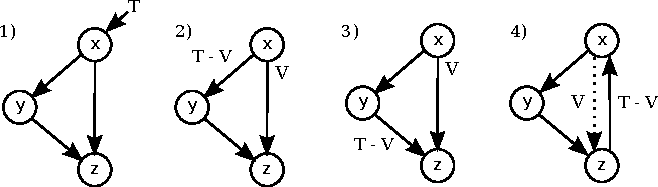
\includegraphics[width=13cm, keepaspectratio]{capitoli/attraversamento/imgs/n_17}
\end{figure}

\begin{enumerate}
    \item $x$ riceve $T$ (TOKEN);
    \item $x$ invia il Token ad $y$ e un Visited ad $y$ e $z$ (supponiamo che il
          Visited verso $z$ abbia ritardi);
    \item $y$ riceve il Token, ed invia Token e Visited all'unico vicino
          disponibile, ossia $z$ (il Visited spedito da $x$ verso $z$ non è ancora
          arrivato);
    \item $z$ riceve il Token da $y$ e manda il Token e Visited verso $x$, dato
          che ancora non ha ricevuto il Visited da $x$. A questo punto $x$ riceve il
          Token da $z$ e capisce che $z$ ha commesso un errore, ignorerà quindi il Token
          ed elimina $z$ dalla lista dei suoi vicini. Nel momento in cui $z$ riceve il
          Visited di $x$, capisce che quello è un vecchio Visited (se $x$ era la prima
          volta che riceveva il Token, non avrebbe mandato un Visited a $z$), a questo
          punto $z$ capisce che ha inviato T al link sbagliato e quindi invia il Token
          ad un'altra strada (se disponibile), altrimenti manda RETURN verso $y$.
\end{enumerate}
Quindi il protocollo funziona anche senza i messaggi di "ACK", ma ammettiamo la
possibilità di inviare T ad un nodo che lo ha già ricevuto, quindi la
possibilità di sbagliare.\\
In questo caso $z$ se avesse ricevuto il VISITED da $x$ avrebbe cambiato stato
in Available ed avrebbe eliminato $x$ dal suo insieme degli Unvisited. A questo
punto in ricezione del messaggio $T$ di $y$ avrebbe avuto l'insieme degli
Unvisited Vuoto, e quindi avrebbe inviato un RETURN verso $y$.


\textbf{Andiamo ora ad analizzare il numero di messaggi utilizzati:}
\begin{itemize}
    \item \#$T$ e \#RETURN corretti = $2(n-1)$
          \begin{itemize}
              \item 2 è per i messaggi di T e RETURN
              \item $n-1$ indica tutti i nodi tranne l'iniziatore, poiché
                    l'iniziatore non riceverà nessun messaggio di T e non invia nessun
                    RETURN.
          \end{itemize}
    \item \#$T$ non corretti $\leq 2(m-n+1)$
          \begin{itemize}
              \item Ogni errore costa 1 messaggio, ma nel peggiore dei casi, il
                    ritardo di comunicazione può forzare gli errori ad accadere in ogni
                    arco che conduce al "sender" (back-edge), in alcuni ci possono essere
                    anche due errori, uno in ogni direzione.


                    %In ogni Arco $m$ posso sbagliare ma sicuramente non sbaglierò
                    %ad inviarlo al sender, quindi risparmio $-n+1$. Negli archi è
                    %possibile che si commettano due errori, uno in ogni direzione e
                    %da questo viene il 2.
          \end{itemize}

    \item \#VISITED = $2m - n + 1$, come nel \texttt{DF+}

\end{itemize}

\textbf{Andiamo infine a valutare i costi: }\\
\underline{Messaggi: (si sommano le tre quantità sopra)}
\begin{center}
    $M[$\texttt{DF++}$/R] \leq 4m - n + 1$
\end{center}

\underline{Tempo:}
Andiamo adesso ad effettuare una stima ideale del tempo, ovvero senza
considerare gli errori che commetto. Al costo precedente di $4n-2$ devo togliere
tutti i miglioramenti che applica questo protocollo:
\begin{center}
    $T[$\texttt{DF++}$/R] = 4n - 2 - n - n = 2n - 2$
\end{center}

Dove:
\begin{itemize}
    \item il primo $-n$ è degli ACK tolti;
    \item il secondo $-n$ è dei VISITED che posso inviare in parallelo con $T$ o
          con $RETURN$, nel caso in cui l'entità che riceve $T-V$ abbia l'insieme degli
          UNVISITED vuoto. Faccio questo perché non devo aspettare niente di ritorno
          dalle entità in quanto gli ACK non ci sono più.
\end{itemize}
Se non invio i Visited in parallelo allora il costo del tempo nel caso peggiore
è $3n$.

\textbf{Nel caso in cui chieda direttamente questo protocollo:}
\begin{center}
    $T[$\texttt{DF++}$/R] = n-1 + n-1 = 2n - 2$
\end{center}
Dove:
\begin{itemize}
    \item $n-1$ sono i messaggi di T sia corretti che non. Non contiamo poi i
          Visited perché vengono inviati in parallelo con T.
    \item $(n-1)$ sono i messaggi di Return
\end{itemize}

\section{DF*: Utilizzo di T come Visited Implicito}
Vediamo adesso un ulteriore miglioria applicabile al precedente protocollo: si
possono utilizzare i messaggi di T come messaggi di VISITED impliciti, quindi
nella direzione in cui invio T, non invio VISITED, ma in tutte le altre
direzioni si. Prima ad ogni invio di T si aveva un messaggio di VISITED sullo
stesso link, questo non accade nella miglioria apportata.
%si manda il messaggio di $T$ in parallelo con il messaggio di VISITED; quindi un $T$ corretto indica anche un VISITED.

\begin{figure}[H]
    \centering
    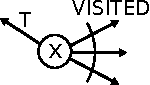
\includegraphics[width=4cm, keepaspectratio]{capitoli/attraversamento/imgs/n_19}
\end{figure}

Il risparmio avverrà su tutte le entità \textbf{tranne} quelle che, quando
vengono raggiunte per la prima volta da un messaggio T, hanno l'insieme degli
UNVISITED già vuoto, ovvero che hanno già tutti i vicini già visitati dal Token
e quindi non lo possono spedire a nessuno, \textbf{sono costrette ad inviare
    immediatamente return. Insieme a questo return l'entità invia ai suoi vicini
    meno quello a cui invia il RETURN i messaggi di visited, non risparmiando
    messaggi}. Sia $f^*$ questo numero di nodi, il numero di messaggi VISITED che
salviamo è $n-f^*$ quindi:

\begin{center}
    $M[$\texttt{DF*}$/R] = 4m - n + 1 - (n - f^*)$
\end{center}

\begin{itemize}
    \item $ 4m - n + 1$: Il costo del protocollo $DF^{++}$ dove avevamo i T
          corretti, i T non corretti, i VISITED ed i RETURN.
    \item $n-f^*$ si ha un risparmio su tutti i nodi tranne esattamente $f^*$.
\end{itemize}
\begin{center}
    $T[$\texttt{DF*}$/R] = 2n - 2$
\end{center}
\begin{center}
    $M[$\texttt{DF*}$/R] = 4m - 2n + f^* + 1$
\end{center}
Al costo del protocollo precedente aggiungo un $-n+f^*$.
\begin{itemize}
    \item Caso migliore: grafo completo (ne risparmio $n-1$);
    \item Caso peggiore: stella (ne risparmio solo $1$).
\end{itemize}
Tra gli stati del protocollo c'è anche Available.

Descrizione del protocollo a parole:
\begin{itemize}
    \item Iniziatore: Si sveglia tramite l'impulso spontaneo, crea l'insieme degli
          UNVISITED, composto da tutti i suoi vicini e ne sceglie uno (lo chiama
          "next"). Invia il token a questo e allo stesso tempo invia il  VISITED a tutto
          il suo vicinato meno quello a cui ha inviato il token.
    \item Idle: Se ricevo T allora creo l'insieme degli unvisited che contiene
          TUTTI i miei vicini (anche il sender), poi richiamo First-Visit. Se
          invece ricevo VISITED allora creo l'insieme degli unvisited che è
          composto da tutti i miei vicini meno il sender. Successivamente divento
          AVAILABLE.
    \item First-Visit: Elimino il sender dal mio insieme degli UNVISITED. Se
          quest'ultimo diventa vuoto, allora \textbf{invio RETURN al mio sender ed allo
              stesso tempo invio VISITED a tutto il mio vicinato meno il sender (a cui ho
              inviato return).} Poi divento DONE. Altrimenti scelgo un vicino dal mio
          insieme e gli invio il Token, mentre invio un VISITED a tutti i miei vicini
          tranne chi mi ha inviato il Token la prima volta e quello a cui ho inviato io
          il Token; successivamente divento VISITED. Altrimenti invio Return a mio
          "padre" ed allo stesso tempo invio il VISITED a tutti i miei vicini meno
          quello a cui ho inviato RETURN.
    \item AVAILABLE: Se ricevo T effettuo la first-visit. Altrimenti se ricevo
          VISITED aggiorno il mio insieme degli unvisited eliminando il vicino che mi ha
          inviato questo messaggio.
    \item VISITED: Se ricevo Visited allora aggiorno il mio insieme degli
          UNVISITED.
\end{itemize}


\section{Traversal in reti specifiche}
\subsection{Alberi}
In un albero la DFS è particolarmente efficiente in termini di messaggi e non ha
bisogno di nessuna miglioria. Infatti in un esecuzione del DF\_TRAVERSAL (il
primo protocollo visto che aveva i messaggi di BackEdge) in un albero, nessun
messaggio di BACKEDGE sarà inviato non essendo presenti cicli. Quindi il numero
totale di messaggi è esattamente $2(n-1)$, stessa cosa per il tempo essendo
sequenziale.
\begin{itemize}
    \item $m = n -1$
\end{itemize}
\begin{center}
    $T[$\texttt{DF}$/R] = 2(n-1) = O(n)$\\
    $M[$\texttt{DF}$/R] = 2(n-1) = O(n)$
\end{center}
%Essendo un albero aciclico, nessun messaggio di BACKEDGE verrà inviato, e non
%c'è bisogno di nessun miglioramento per il costo di entrambi.
\subsection{Anello}
In un anello, ogni nodo ha esattamente due vicini. La DFS in queste reti può
essere applicata tramite la scelta di una direzione da parte dell'iniziatore,
una volta che il messaggio di T ritorna indietro a lui il protocollo termina.
Quindi ogni entità riceve un singolo messaggio di T; il costo sarà O(n).
\begin{itemize}
    \item $m = n$
\end{itemize}
\begin{center}
    $T[$\texttt{DF}$/R] = O(n)$ \\
    $M[$\texttt{DF}$/R] = O(n)$
\end{center}
Si può ottimizzare l'algoritmo scegliendo una direzione di invio.

\subsection{Grafi completi}
\begin{itemize}
    \item $m = O(n^2)$
\end{itemize}
L'esecuzione dell'algoritmo $DF^*$ richiederebbe O($n^2)$ messaggi. Un miglior
protocollo potrebbe essere quello di fare in modo che l'initiator invii il token
t sequenzialmente a tutti i suoi vicini uno alla volta; ogni entità ritorna poi
il token all'initiator senza propagarlo a nessun altro. In questo caso il costo
dei messaggi e del tempo sarebbe $2(n-1)$.
\begin{center}
    $T[$\texttt{DF}$/R] = 2(n-1)$\\
    $M[$\texttt{DF}$/R] = 2(n-1)$
\end{center}
Un'altra metodologia sarebbe quella di organizzare il grafo a stella:
\begin{center}
    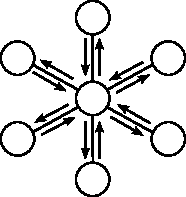
\includegraphics[scale=1]{capitoli/attraversamento/imgs/n_20}
\end{center}
\begin{center}
    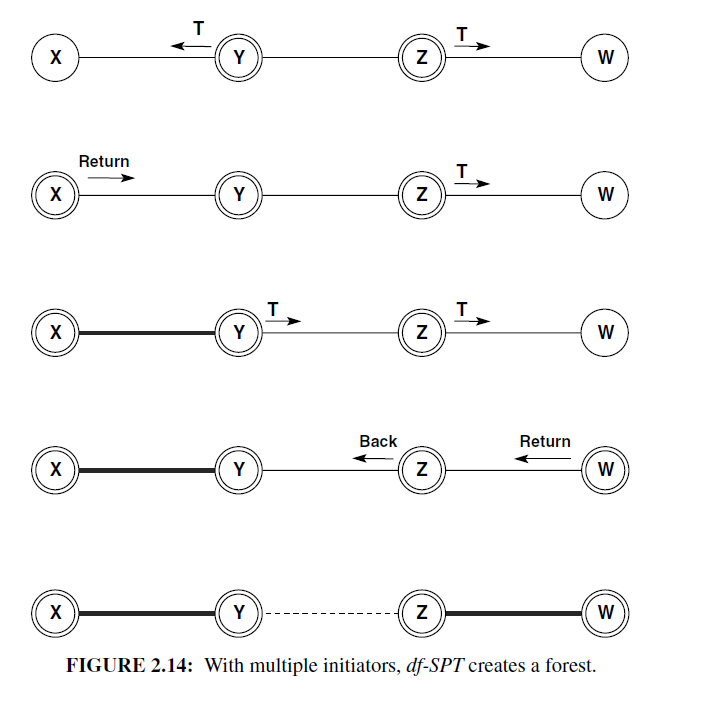
\includegraphics[scale=0.6]{capitoli/attraversamento/imgs/asd.png}
\end{center}
